% Se pre-carga la información del estudiante sólo para poder emplear el macro de
% selección de versión (digital o impresa)
% ===============================================================================
% El estudiante debe llenar sus datos en esta sección para que la plantilla los 
% auto-importe y genere automáticamente las páginas de portada y de firmas 
% autorizadas.
% ===============================================================================
% Datos del estudiante:
% -------------------------------------------------------------------------------
% Nombre completo
\def \nombreestudiante {Erick Stiv Junior Guerra Muñoz}
% Carné
\def \uvgcarne {21781}
% Facultad
\def \uvgfacultad {Ingeniería}
% Carrera
\def \uvgcarrera {Ingeniería en Ciencias de la Computación y Tecnologías de la Información}

% Datos del trabajo:
% -------------------------------------------------------------------------------
% Título completo
\def \titulotesis {Ciudadano Digital: La Inteligencia Artifcial como herramienta de acompañamiento informal en educación sobre ciudadanía y valores morales.}
% Año de entrega
\def \anoentrega {2025}
% Asesor
\def \nombreasesor {MA. Luis Furlán}

% Datos del tribunal examinador:
% -------------------------------------------------------------------------------
% Nombre del primer examinador
\def \nombreprimerex {MSc. Douglas Barrios}
% Nombre del segundo examinador
\def \nombresegundoex {PhD. Gabriel Barrientos}
% Año de aprobación
\def \anoaprobacion {2025}

% Capítulos pre-definidos
% -------------------------------------------------------------------------------
% Comentar las líneas de las secciones que desean omitirse, por defecto se 
% se incluyen todas.


% Formato y estilo de la plantilla
% -------------------------------------------------------------------------------
% Modo impresión: Puede des-comentar la siguiente línea para generar un documento pdf sin la portada, para cuando se desee imprimir el documento para encuadernación
%\def \printver {Versión del documento para impresión}

% Portada: Puede cambiarse la imagen en la portada al cambiar el nombre del 
% archivo siguiente. NOTA: debe tener la suficiente resolución para cubrir el área
% designada
\def \imagenportada {plantilla/portadacit.jpg}

% Referencias: Puede des-comentar la siguiente línea para utilizar el formato de referencias APA
%\def \usarAPA {Usar formato APA}

% Párrafo: Puede comentar la siguiente línea si desea emplear un formato de 
% párrafo distinto al establecido por defecto
\def \parpordefecto {Formato de párrafo por defecto}

% Capítulos y secciones: Puede des-comentar la siguiente línea para establecer el
% formato de los capítulos y secciones bajo el estándar original de UVG para
% trabajos de graduación. Este incluye: capítulos con numeración romana, secciones
% con letras mayúsculas, sub-secciones con números y sub-sub-secciones con letras
% minúsculas
%\def \capsecuvg {Formato UVG para capítulos y secciones}

\ifdefined\printver
    \documentclass[11pt, letterpaper, twoside, openright]{report}
\else
    \documentclass[11pt, letterpaper]{report}
\fi

% Eliminar la opción de twoside y openright si se desea generar la versión
% digital del documento en lugar de la versión impresa
%\documentclass[11pt, letterpaper, twoside, openright]{report}
\usepackage[spanish, es-nodecimaldot, es-noquoting]{babel}
% cambiar a spanish, mexico si se quiere emplear tabla en lugar de cuadro
\selectlanguage{spanish}
\usepackage[utf8]{inputenc}
\usepackage[T1]{fontenc}

\title{Plantilla para Trabajos de Graduación IE-MT 2019v3}
\author{MSc. Miguel Zea}
\date{\today}

% Información del estudiante en el archivo datos_estudiante.tex
% ===============================================================================
% El estudiante debe llenar sus datos en esta sección para que la plantilla los 
% auto-importe y genere automáticamente las páginas de portada y de firmas 
% autorizadas.
% ===============================================================================
% Datos del estudiante:
% -------------------------------------------------------------------------------
% Nombre completo
\def \nombreestudiante {Erick Stiv Junior Guerra Muñoz}
% Carné
\def \uvgcarne {21781}
% Facultad
\def \uvgfacultad {Ingeniería}
% Carrera
\def \uvgcarrera {Ingeniería en Ciencias de la Computación y Tecnologías de la Información}

% Datos del trabajo:
% -------------------------------------------------------------------------------
% Título completo
\def \titulotesis {Ciudadano Digital: La Inteligencia Artifcial como herramienta de acompañamiento informal en educación sobre ciudadanía y valores morales.}
% Año de entrega
\def \anoentrega {2025}
% Asesor
\def \nombreasesor {MA. Luis Furlán}

% Datos del tribunal examinador:
% -------------------------------------------------------------------------------
% Nombre del primer examinador
\def \nombreprimerex {MSc. Douglas Barrios}
% Nombre del segundo examinador
\def \nombresegundoex {PhD. Gabriel Barrientos}
% Año de aprobación
\def \anoaprobacion {2025}

% Capítulos pre-definidos
% -------------------------------------------------------------------------------
% Comentar las líneas de las secciones que desean omitirse, por defecto se 
% se incluyen todas.


% Formato y estilo de la plantilla
% -------------------------------------------------------------------------------
% Modo impresión: Puede des-comentar la siguiente línea para generar un documento pdf sin la portada, para cuando se desee imprimir el documento para encuadernación
%\def \printver {Versión del documento para impresión}

% Portada: Puede cambiarse la imagen en la portada al cambiar el nombre del 
% archivo siguiente. NOTA: debe tener la suficiente resolución para cubrir el área
% designada
\def \imagenportada {plantilla/portadacit.jpg}

% Referencias: Puede des-comentar la siguiente línea para utilizar el formato de referencias APA
%\def \usarAPA {Usar formato APA}

% Párrafo: Puede comentar la siguiente línea si desea emplear un formato de 
% párrafo distinto al establecido por defecto
\def \parpordefecto {Formato de párrafo por defecto}

% Capítulos y secciones: Puede des-comentar la siguiente línea para establecer el
% formato de los capítulos y secciones bajo el estándar original de UVG para
% trabajos de graduación. Este incluye: capítulos con numeración romana, secciones
% con letras mayúsculas, sub-secciones con números y sub-sub-secciones con letras
% minúsculas
%\def \capsecuvg {Formato UVG para capítulos y secciones}
% ================================================================================
% En este archivo se colocan opciones adicionales para modificar el formato de la
% plantilla, para emplearse en otros tipos de documentos que no sean trabajos de
% graduación. Si usted está trabajando su tesis, NO modifique este archivo
% ================================================================================
% Capítulos pre-definidos
% --------------------------------------------------------------------------------
% Comentar las líneas de las secciones que desean omitirse, por defecto se 
% se incluyen todas.
\def \CAPportada {Portada}
\def \CAPcaratula {Caratula}
\def \CAPcaratula {Caratula}
\def \CAPfirmas {Hoja de firmas}

%Opcionales
% Dedicatoria / Reconocimiento (opcional)
% \def \CAPdedicatoria {Dedicatoria}
% \def \CAPprefacio {Prefacio}

\def \CAPresumen {Resumen}
% Abstract
\def \CAPabstract {Resumen}

%Tablas de contenido
\def \CAPindice {Índice general}
\def \CAPcuadros {Listado de tablas}
\def \CAPalgoritmos {Listado de algoritmos}
% \def \CAPfiguras {Listado de figuras}
% \def \CAPglosario {Glosario}

\def \CAPintroduccion {Introducción}

%Opcionales
\def \CAPjustificacion {Justificación}
% \def \CAPantecedentes {Antecedentes}

\def \CAPobjetivos {Objetivos}

%Opcionales
% \def \CAPalcance {Alcances}

\def \CAPmarcoteorico {Marco teórico}
% Metodología
\def \CAPmetodologia {Metodología}
% Resultados
\def \CAPresultados {Resultados}
% Discusión
\def \CAPdiscusion {Discusión}
\def \CAPconclusiones {Conclusiones}
%\def \CAPrecomendaciones {Recomendaciones}
\def \CAPbibliografia {Bibliografía}

% Opcionales
% \def \CAPanexos {Anexos}
% Apéndice
% \def \CAPapendice {Apéndice}

% ==============================================================================
% DEFINICIÓN DE PAQUETES
% ==============================================================================
\usepackage{xcolor}
\usepackage{amsfonts}
\usepackage{amsmath}
\usepackage{amssymb}
\usepackage{amsthm}
\usepackage{amsfonts}
\usepackage{mathtools}
\usepackage{graphicx}
\usepackage{xfrac}
\usepackage{float}
\usepackage{mathtools}
\usepackage[hypertexnames=false]{hyperref}
% \usepackage{bookmark}
\usepackage[font=small]{caption}
\usepackage{subcaption}
%\usepackage{csquotes}
\usepackage{xpatch}
\usepackage{emptypage}
\usepackage{hyphenat}
\usepackage{fancyhdr}
\usepackage[backend=biber, style=ieee]{biblatex}
\ifdefined\usarAPA 
    \usepackage[backend=biber, style=apa]{biblatex}
\fi
\addbibresource{m-bibliografia.bib}

\usepackage[percent]{overpic}

\usepackage{chngcntr}

\ifdefined\CAPglosario
	%\usepackage[toc]{glossaries}
	\usepackage[numberedsection]{glossaries}
	\makeglossaries
    \newglossaryentry{latex}
{
    name=latex,
    description={Es un lenguaje de marcado adecuado especialmente para la creación de documentos científicos}
} 
 
\newglossaryentry{formula}
{
    name=fórmula,
    description={Una expresión matemática} 
}
\fi

% ==============================================================================
% MÁRGENES Y FORMATO GENERALES
% ==============================================================================
\usepackage[top=1in, left=1.5in, right=1in, bottom=1in]{geometry}
%Options: Sonny, Lenny, Glenn, Conny, Rejne, Bjarne, Bjornstrup
\usepackage[Sonny]{fncychap}

% ==============================================================================
% DEFINICIONES DE LA PLANTILLA
% ==============================================================================
\graphicspath{ {figuras/} }
\definecolor{uvg-green}{RGB}{17,71,52}
\newcommand{\defaultparformat}[1]{
	{\setlength{\parskip}{2ex}
     \input{#1}}
}
\ifdefined\capsecuvg
	\renewcommand\thechapter{\Roman{chapter}}
    \renewcommand\thesection{\Alph{section}}
	\renewcommand\thesubsection{\arabic{subsection}}
    \renewcommand\thesubsubsection{\alph{subsubection}}
\fi
\counterwithout{figure}{chapter}
\counterwithout{table}{chapter}
\counterwithout{equation}{chapter}

\newcommand{\blankpage}{
\newpage
\thispagestyle{empty}
\mbox{}
\newpage
}
% ==============================================================================

% Comandos definidos por el usuario en el archivo comandos_usuario.tex
\input{2-paquetes_y_comandos_usuario}

% ==============================================================================
% CUERPO DEL TRABAJO
% ==============================================================================
\pagestyle{headings}
\begin{document}

% ==============================================================================
% PORTADA
% ==============================================================================
\ifdefined\printver
    \let\CAPportada\undefined
\fi 

\ifdefined\CAPportada
    \cleardoublepage\phantomsection
    % \pdfbookmark{Portada}{toc}
	\newgeometry{left=3cm, bottom=0in, top=1in, right=3cm}
	\pagecolor{uvg-green}
	\thispagestyle{empty}

	\color{white}
	\noindent \hrulefill \par
	\vspace{0.1in}
	\noindent \Huge \nohyphens{\titulotesis} \par
	\noindent \hrulefill \par
	\noindent
	\LARGE \nombreestudiante

	\begin{figure}[b!]
    	%\makebox[\textwidth]{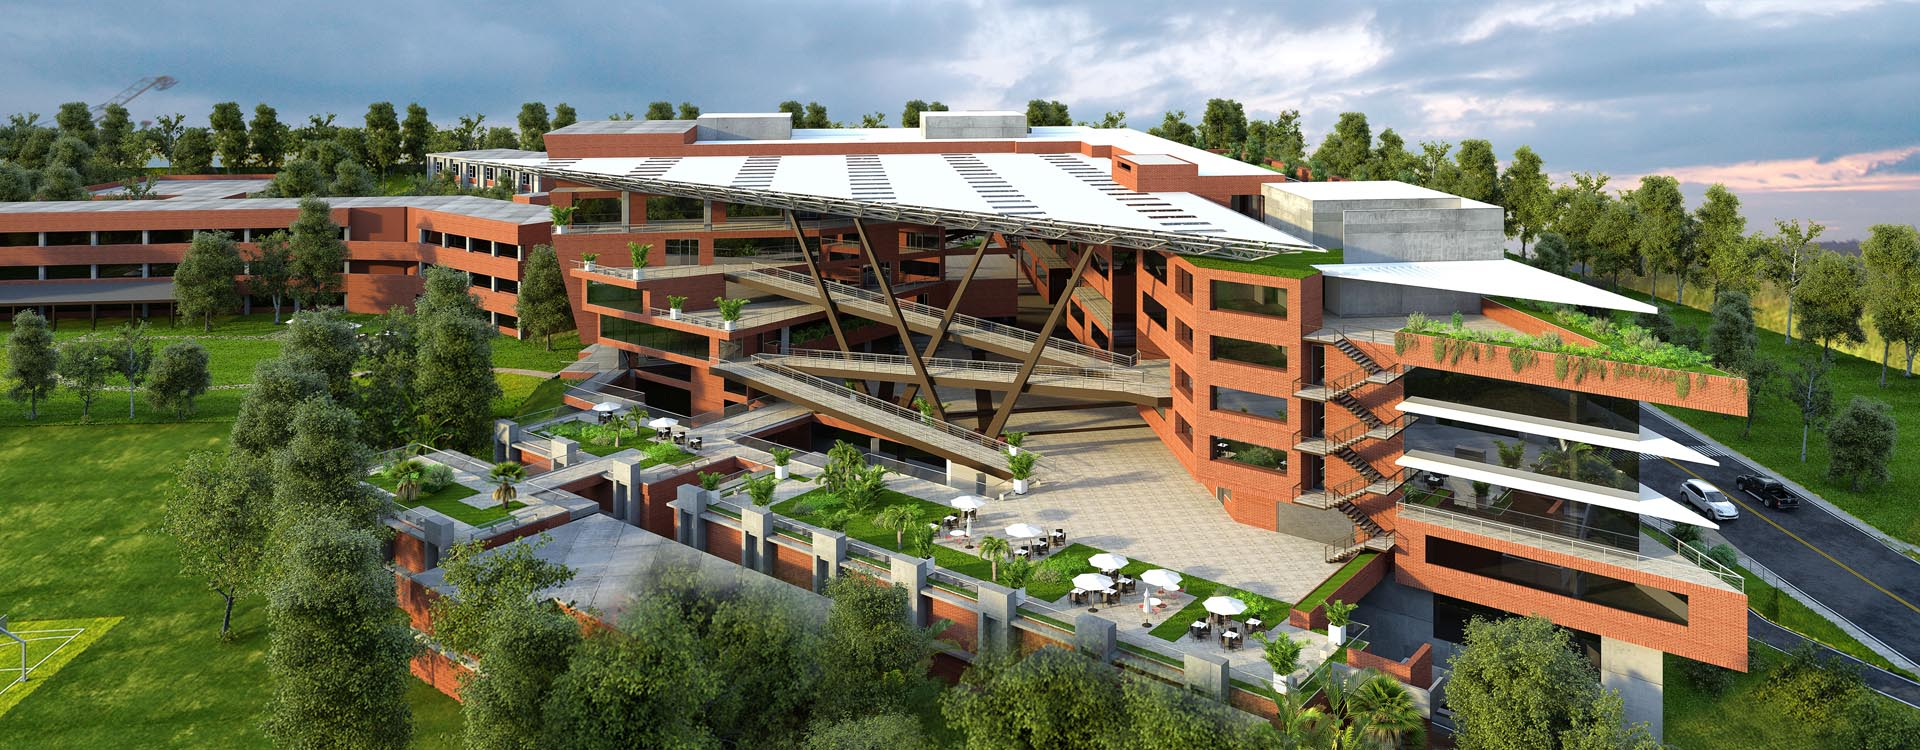
\includegraphics[height=13.25cm]{plantilla/portadacit.jpg}}
    	\makebox[\textwidth]{
    		\begin{overpic}[height=13.25cm]{\imagenportada}
     		\put(63,0){
\includegraphics[height=1.15in]{plantilla/fondologo_grande.png}}  
  			\put(64.5,2){
\includegraphics[height=0.55in]{plantilla/logoUVGblanco.eps}} 
        	\end{overpic}
    	}
    	%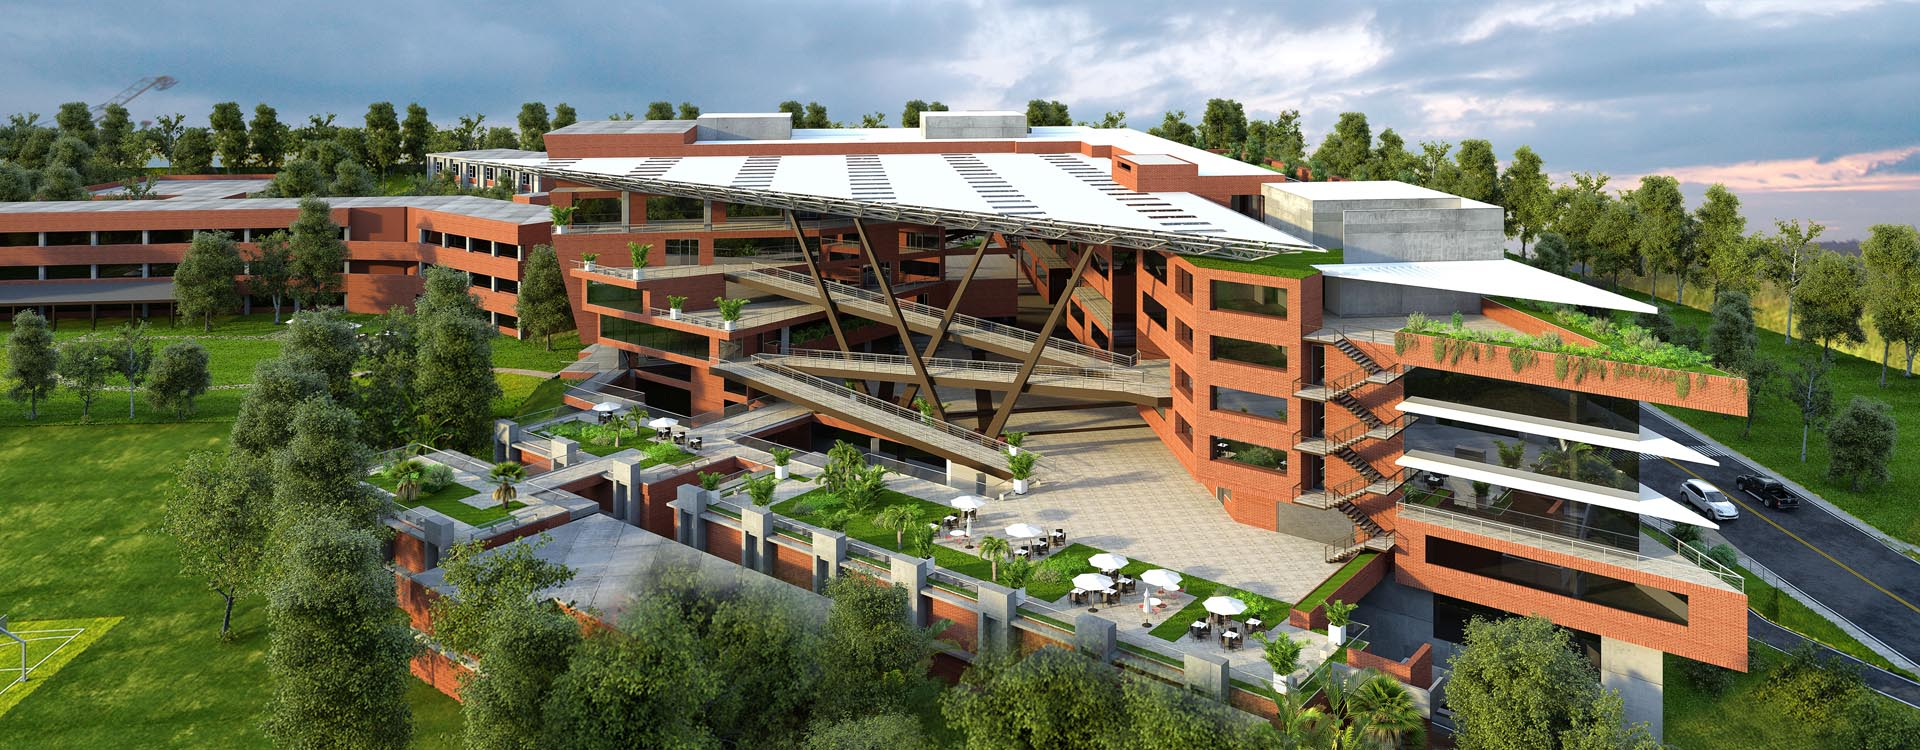
\includegraphics[height=13.25cm]{plantilla/portadacit.jpg}
	\end{figure}
	\restoregeometry
\fi

% ==============================================================================
% PRIMERAS PÁGINAS (Carátulas más hojas de guarda)
% ==============================================================================
\ifdefined\CAPcaratula
	\newpage
    \cleardoublepage\phantomsection
    % \pdfbookmark{Carátula}{toc}
	\pagecolor{white}
	\color{black}
	\setcounter{page}{1}
	\pagenumbering{roman}
	\thispagestyle{empty}
	\begin{center}
		\LARGE UNIVERSIDAD DEL VALLE DE GUATEMALA\\
		\LARGE Facultad de \uvgfacultad \\[0.75cm]
	\end{center}
	\begin{figure}[h]
		\begin{center}
		
\includegraphics[height=5.5 cm]{plantilla/escudoUVGnegro.eps}
		\vspace{0.5in}
		\end{center}
	\end{figure}
	\begin{center}
		\Large \textbf{\nohyphens{\titulotesis}} \\
		%\LARGE \textbf{\titulotesis} \\
		\vfill
		\Large \nohyphens{Trabajo de graduación presentado por \nombreestudiante \ para optar al grado académico de Licenciado en \uvgcarrera} \\
		\vfill
		\large Guatemala, \\
		\vspace{1em}
		\anoentrega
	\end{center}
    
    \ifdefined\printver	
	    \blankpage
	    \blankpage
	    
	    \newpage
	    \cleardoublepage\phantomsection
	    \pagecolor{white}
    	\color{black}
    	\setcounter{page}{1}
    	\pagenumbering{roman}
    	\thispagestyle{empty}
    	\begin{center}
    		\LARGE UNIVERSIDAD DEL VALLE DE GUATEMALA\\
    		\LARGE Facultad de \uvgfacultad \\[0.75cm]
    	\end{center}
    	\begin{figure}[h]
    		\begin{center}
    		
\includegraphics[height=5.5 cm]{plantilla/escudoUVGnegro.eps}
    		\vspace{0.5in}
    		\end{center}
    	\end{figure}
    	\begin{center}
    		\Large \textbf{\nohyphens{\titulotesis}} \\
    		%\LARGE \textbf{\titulotesis} \\
    		\vfill
    		\Large \nohyphens{Trabajo de graduación presentado por \nombreestudiante \ para optar al grado académico de Licenciado en \uvgcarrera} \\
    		\vfill
    		\large Guatemala, \\
    		\vspace{1em}
    		\anoentrega
    	\end{center}
    \fi
\fi

% ==============================================================================
% HOJA DE FIRMAS
% ==============================================================================
\ifdefined\CAPfirmas
	\newpage
	\cleardoublepage\phantomsection
	\thispagestyle{empty}
	\vspace*{0.5in}
	\large Vo.Bo.:\\[1cm]
	\begin{center}
		(f) \rule[1pt]{4 in}{1pt}\\
		\nombreasesor
	\end{center}
	\vspace{1in}

	Tribunal Examinador:\\[1cm]
	\begin{center}
		(f) \rule[1pt]{4 in}{1pt}\\
		\nombreasesor \\[1in]
		(f) \rule[1pt]{4 in}{1pt}\\
		\nombreprimerex \\[1in]
		(f) \rule[1pt]{4 in}{1pt}\\
		\nombresegundoex
	\end{center}
	\vspace{1in}

	Fecha de aprobación: Guatemala, \rule[1pt]{0.5 in}{1pt} de \rule[1pt]{1 in}{1pt} de \anoaprobacion.
	\normalsize
\fi

% Comentar para formato estilo libro en la numeración de páginas (NO 
% compatible con la guía UVG 2019)
\pagestyle{plain}
% ==============================================================================
% CONTENIDO DEL TRABAJO
% ==============================================================================
% PREFACIO
% ------------------------------------------------------------------------------
\ifdefined\CAPprefacio
	\newpage
	\cleardoublepage\phantomsection
    \chapter*{Prefacio}
    \ifdefined\parpordefecto
    	\defaultparformat{a-prefacio}
    \else
    	Lorem ipsum dolor sit amet, consectetur adipiscing elit. Cras vitae eleifend ipsum, ut mattis nunc. Pellentesque ac hendrerit lacus. Cras sollicitudin eget sem nec luctus. Vivamus aliquet lorem id elit venenatis pellentesque. Nam id orci iaculis, rutrum ipsum vel, porttitor magna. Etiam molestie vel elit sed suscipit. Proin dui risus, scelerisque porttitor cursus ac, tempor eget turpis. Aliquam ultricies congue ligula ac ornare. Duis id purus eu ex pharetra feugiat. Vivamus ac orci arcu. Nulla id diam quis erat rhoncus hendrerit. Class aptent taciti sociosqu ad litora torquent per conubia nostra, per inceptos himenaeos. Sed vulputate, metus vel efficitur fringilla, orci ex ultricies augue, sit amet rhoncus ex purus ut massa. Nam pharetra ipsum consequat est blandit, sed commodo nunc scelerisque. Maecenas ut suscipit libero. Sed vel euismod tellus.

Proin elit tellus, finibus et metus et, vestibulum ullamcorper est. Nulla viverra nisl id libero sodales, a porttitor est congue. Maecenas semper, felis ut rhoncus cursus, leo magna convallis ligula, at vehicula neque quam at ipsum. Integer commodo mattis eros sit amet tristique. Cras eu maximus arcu. Morbi condimentum dignissim enim non hendrerit. Sed molestie erat sit amet porttitor sagittis. Maecenas porttitor tincidunt erat, ac lacinia lacus sodales faucibus. Integer nec laoreet massa. Proin a arcu lorem. Donec at tincidunt arcu, et sodales neque. Morbi rhoncus, ligula porta lobortis faucibus, magna diam aliquet felis, nec ultrices metus turpis et libero. Integer efficitur erat dolor, quis iaculis metus dignissim eu.
    \fi
    \addcontentsline{toc}{chapter}{Prefacio}
\fi

% ÍNDICE GENERAL
% ------------------------------------------------------------------------------
\ifdefined\CAPindice
	\newpage
    \cleardoublepage\phantomsection
	\renewcommand{\contentsname}{Índice}
    %\phantomsection
    \pdfbookmark{\contentsname}{toc}
    %\pdfbookmark{Índice}{toc}
	\tableofcontents
\fi

% LISTADO DE FIGURAS
% ------------------------------------------------------------------------------
\ifdefined\CAPfiguras
	\newpage
    \cleardoublepage\phantomsection
	\renewcommand{\listfigurename}{Lista de figuras}
	\listoffigures
	\addcontentsline{toc}{chapter}{Lista de figuras}
\fi

% LISTADO DE CUADROS
% ------------------------------------------------------------------------------
\ifdefined\CAPcuadros
	\newpage
    \cleardoublepage\phantomsection
	\renewcommand{\listtablename}{Lista de cuadros}
	\listoftables
	\addcontentsline{toc}{chapter}{Lista de cuadros}
\fi

% RESUMEN
% ------------------------------------------------------------------------------
\ifdefined\CAPresumen
	\newpage
    \cleardoublepage\phantomsection
	\chapter*{Resumen}
	\ifdefined\parpordefecto
		\defaultparformat{b-resumen}
	\else
		Lorem ipsum dolor sit amet, consectetur adipiscing elit. Cras vitae eleifend ipsum, ut mattis nunc. Pellentesque ac hendrerit lacus. Cras sollicitudin eget sem nec luctus. Vivamus aliquet lorem id elit venenatis pellentesque. Nam id orci iaculis, rutrum ipsum vel, porttitor magna. Etiam molestie vel elit sed suscipit. Proin dui risus, scelerisque porttitor cursus ac, tempor eget turpis. Aliquam ultricies congue ligula ac ornare. Duis id purus eu ex pharetra feugiat. Vivamus ac orci arcu. Nulla id diam quis erat rhoncus hendrerit. Class aptent taciti sociosqu ad litora torquent per conubia nostra, per inceptos himenaeos. Sed vulputate, metus vel efficitur fringilla, orci ex ultricies augue, sit amet rhoncus ex purus ut massa. Nam pharetra ipsum consequat est blandit, sed commodo nunc scelerisque. Maecenas ut suscipit libero. Sed vel euismod tellus.

Proin elit tellus, finibus et metus et, vestibulum ullamcorper est. Nulla viverra nisl id libero sodales, a porttitor est congue. Maecenas semper, felis ut rhoncus cursus, leo magna convallis ligula, at vehicula neque quam at ipsum. Integer commodo mattis eros sit amet tristique. Cras eu maximus arcu. Morbi condimentum dignissim enim non hendrerit. Sed molestie erat sit amet porttitor sagittis. Maecenas porttitor tincidunt erat, ac lacinia lacus sodales faucibus. Integer nec laoreet massa. Proin a arcu lorem. Donec at tincidunt arcu, et sodales neque. Morbi rhoncus, ligula porta lobortis faucibus, magna diam aliquet felis, nec ultrices metus turpis et libero. Integer efficitur erat dolor, quis iaculis metus dignissim eu.
	\fi
	\addcontentsline{toc}{chapter}{Resumen}
\fi

% ABSTRACT
% ------------------------------------------------------------------------------
\ifdefined\CAPabstract
	\newpage
    \cleardoublepage\phantomsection
	\chapter*{Abstract}
	\ifdefined\parpordefecto
		\defaultparformat{c-abstract}
	\else
		This is an abstract of the study developed under the
	\fi
	\addcontentsline{toc}{chapter}{Abstract}
\fi

% INTRODUCCIÓN
% ------------------------------------------------------------------------------
\ifdefined\CAPintroduccion
	\newpage
	\cleardoublepage
	\pagenumbering{arabic}
	\setcounter{page}{1}
	\chapter{Introducción}
	\ifdefined\parpordefecto
		\defaultparformat{d-introduccion}
	\else
		Lorem ipsum dolor sit amet, consectetur adipiscing elit. Quisque eget consequat risus. Praesent a quam lacinia, consequat eros id, auctor tellus. Phasellus a dapibus arcu, vitae luctus leo. Aliquam erat volutpat. Suspendisse ac velit quam. Nullam risus nibh, lobortis vehicula elit non, pellentesque volutpat odio. Donec feugiat porta sapien gravida interdum. Cras odio nunc, lobortis sed pellentesque imperdiet, facilisis eu quam. Praesent pharetra, orci at tincidunt lacinia, neque nulla ornare lacus, ut malesuada elit risus non mi. Fusce pellentesque vitae sapien sed mollis. Curabitur viverra at nulla vitae porta. In et mauris lorem.

Vestibulum faucibus fringilla justo, eget facilisis elit convallis sit amet. Morbi nisi metus, hendrerit quis pellentesque non, faucibus at leo. Proin consectetur, est vel facilisis facilisis, arcu felis vestibulum quam, et fringilla metus neque at enim. Nunc justo mauris, egestas quis maximus eget, viverra vehicula nunc. Fusce eu nulla elementum, condimentum diam at, aliquam leo. Nullam sed sodales enim, eu imperdiet risus. Aliquam ornare augue leo, fringilla mattis nunc facilisis eget. Nam faucibus, libero a aliquet fermentum, magna arcu ultrices lacus, a placerat tortor turpis ut purus.

Integer eget ligula non metus egestas rutrum sit amet ut tellus. Aliquam vel convallis est, eu sodales leo. Proin consequat nisi at nunc malesuada gravida. Aliquam erat volutpat. Aliquam finibus interdum dignissim. Etiam feugiat hendrerit nisl, hendrerit feugiat ex malesuada in. Cras tempus eget arcu vitae congue. Ut non tristique mauris. Vivamus in mattis ipsum. Cras bibendum, enim bibendum commodo accumsan, ligula nulla porttitor ex, et pharetra eros nisl eget ex. Morbi at semper arcu. Curabitur massa sem, maximus id metus ut, molestie tempus quam. Vivamus dictum nunc vitae elit malesuada convallis. Donec ac semper turpis, non scelerisque justo. In congue risus id vulputate gravida. Nam ut mattis sapien.
	\fi
\fi

% ANTECEDENTES
% ------------------------------------------------------------------------------
\ifdefined\CAPantecedentes
	\newpage
	\chapter{Antecedentes}
	\ifdefined\parpordefecto
    	\defaultparformat{e-antecedentes}
    \else
    	Puede encontrarse un trabajo similar en \cite{hoover2010bio} o bien \cite{park2014design}
    \fi  
\fi

% JUSTIFICACIÓN
% ------------------------------------------------------------------------------
\ifdefined\CAPjustificacion
	\newpage
	\chapter{Justificación}
	\ifdefined\parpordefecto
		\defaultparformat{f-justificacion}
	\else
		hgjhjjhvjvhgvjhgvjhg
\begin{table}[h]
\begin{tabular}{|l|l|l|l|l|}
\hline
12       & $3.2$  & $3.43$    & 23    & 13      \\ \hline
aasdasdd & asd & ssdssa & ssdas & asdasda \\ \hline
         &     &        &       &         \\ \hline
         &     &        &       &         \\ \hline
\end{tabular}
\caption[Pruebas preliminares]{Pruebas preliminares. Este cuadro corresponde a las pruebas realizadas durante blabla} 
\label{cuadro:pritabla}
\end{table}
	\fi
\fi

% OBJETIVOS
% ------------------------------------------------------------------------------
\ifdefined\CAPobjetivos
	\newpage
	\chapter{Objetivos}
	\ifdefined\parpordefecto
		\defaultparformat{g-objetivos}
	\else
		\section{Objetivo general}
Lorem ipsum dolor sit amet, consectetur adipiscing elit. Praesent eu lectus tincidunt, malesuada lorem nec, accumsan ligula.

\section{Objetivos específicos}
\begin{itemize}
\item Nulla ut ex ut mauris pretium elementum.
\item Suspendisse malesuada lectus nec nisi iaculis, in luctus turpis laoreet.
\item In efficitur nisl vitae justo interdum, vitae condimentum lectus maximus.
\item Morbi quis libero sit amet velit commodo tristique eu sed nisl.
\end{itemize}
	\fi
\fi

% ALCANCE
% ------------------------------------------------------------------------------
\ifdefined\CAPalcance
	\newpage
	\chapter{Alcance}
	\ifdefined\parpordefecto
    	\defaultparformat{h-alcance}
    \else
    	Podemos usar \Gls{latex} para escribir de forma ordenada una \gls{formula} matemática. 
    \fi 
\fi

% MARCO TEÓRICO
% ------------------------------------------------------------------------------
\ifdefined\CAPmarcoteorico
	\newpage
	\chapter{Marco teórico}
	\ifdefined\parpordefecto
		\defaultparformat{i-marco_teorico}
	\else
		

Lorem ipsum dolor sit amet, consectetur adipiscing elit. Nam vestibulum, nisl in semper semper, urna ex vehicula enim, eu luctus est velit a est. Class aptent taciti sociosqu ad litora torquent per conubia nostra, per inceptos himenaeos. Mauris et dui ipsum. Praesent tempus vestibulum augue eget venenatis. Curabitur sollicitudin erat vel leo finibus tincidunt. Nullam ullamcorper, risus eu varius venenatis, nibh ligula egestas ante, vel commodo ipsum ante ac enim. Sed iaculis pharetra magna. Duis sit amet augue vitae mi lobortis tristique. Suspendisse non euismod quam. Donec a tincidunt lacus. Aliquam metus quam, rutrum non libero vel, interdum molestie turpis.

Maecenas enim ligula, placerat quis purus eu, pretium tempor justo. Pellentesque accumsan sem eget mattis scelerisque. Ut consectetur lorem dui, a efficitur lectus tincidunt id. Aliquam quis fermentum elit. Pellentesque facilisis semper sem, vitae ornare purus. Morbi ultricies, orci sit amet porta facilisis, ex justo varius elit, viverra euismod sapien enim vel justo. Sed felis mi, feugiat quis molestie ac, gravida sed nunc. Proin elementum, augue quis ultrices dictum, nisl magna pharetra magna, ut ullamcorper diam dolor in elit. In hac habitasse platea dictumst. Suspendisse hendrerit leo non ex ornare mattis. Fusce hendrerit imperdiet nisl in viverra. Proin non turpis ut sapien pulvinar aliquam eu aliquet turpis. Etiam commodo tellus nec ipsum sodales feugiat. Morbi vel pulvinar nibh, nec varius turpis.

Donec a libero vel lacus tincidunt dapibus. Nullam et leo volutpat dui feugiat volutpat vel lacinia ante. Donec finibus risus at facilisis gravida. Cras efficitur felis elementum purus finibus ultricies. Nunc sit amet diam egestas, blandit mauris nec, gravida nisi. In a arcu eu nunc mattis dictum sed placerat arcu. Morbi sit amet venenatis lectus, vitae lobortis nisl. Pellentesque id mattis magna, et convallis leo. Maecenas ultricies hendrerit quam vel ornare. Pellentesque fermentum aliquet velit quis malesuada. Proin commodo, est ultrices rhoncus scelerisque, massa nulla congue tellus, ut porta ante ante vitae nisl. In pharetra quam et urna dictum scelerisque. Aliquam in metus velit. Phasellus aliquet velit molestie, tincidunt purus vestibulum, aliquet odio. Sed augue odio, scelerisque non mi et, pulvinar bibendum justo. Vestibulum sed hendrerit urna.

Donec a lacus quis mi volutpat mollis ac ut lorem. Nulla porta venenatis faucibus. Fusce metus lectus, ullamcorper vel risus laoreet, consequat faucibus sapien. Donec vitae ultrices mauris, dignissim sodales eros. Integer hendrerit elementum ipsum a vestibulum. Vivamus in pretium orci. Fusce condimentum, nibh tempor sagittis laoreet, dui erat luctus neque, a ultrices arcu mauris eget massa. Duis quis ante metus. Interdum et malesuada fames ac ante ipsum primis in faucibus.

Vestibulum laoreet tortor enim, nec tristique turpis dapibus id. Nam quis erat ac nibh imperdiet placerat et a sapien. Aliquam sollicitudin, leo a aliquam vestibulum, lectus eros maximus justo, eu tincidunt justo ipsum non risus. Curabitur ultrices mi vitae elit venenatis, vel semper orci consequat. Nulla ac mauris vitae orci tincidunt mattis. Mauris risus justo, luctus non diam in, dapibus scelerisque eros. Donec fringilla risus sit amet sapien tempus viverra. Quisque quis justo ut enim gravida mollis in vulputate libero. Maecenas auctor accumsan turpis, id dapibus odio aliquet sit amet. Sed feugiat libero eget facilisis finibus. Sed vitae nulla nec felis porta convallis a in purus. Integer finibus efficitur lorem at aliquet. Etiam venenatis velit non tempus porttitor.

Suspendisse tincidunt a orci sed vehicula. Aenean ac mauris enim. Duis vitae fringilla augue. Mauris fringilla neque ac nunc aliquet porta. Praesent quis elit convallis, vehicula leo a, tincidunt leo. Curabitur vitae ligula non leo faucibus cursus sit amet nec ex. Proin mollis lectus in odio aliquet, eu tristique lacus aliquet. Aliquam auctor eget lorem quis porttitor. Duis sagittis eros ac diam ornare, id auctor elit cursus. Morbi vel dolor et odio laoreet ornare. Cras sit amet pretium neque. Mauris vestibulum ante sit amet eros rutrum eleifend ac a sapien. Nullam vitae convallis eros. Proin blandit a nulla nec hendrerit. Fusce ultrices, nibh in mattis consequat, nisi libero rutrum lacus, vitae vulputate lorem tellus vitae enim.

Quisque feugiat felis diam. Maecenas elementum, neque ut ornare tristique, nulla sem semper diam, vel imperdiet purus arcu sit amet magna. Nullam tempus eleifend ultrices. Maecenas pharetra ac leo eget mattis. Donec suscipit arcu justo, ac finibus diam scelerisque sit amet. Nulla et porta urna. Donec vel ultrices lectus. Quisque id molestie tellus. Vivamus vitae elit sit amet ipsum tincidunt sodales eget eget tortor. Quisque vitae placerat ipsum. Donec malesuada ipsum a consectetur venenatis.

Morbi pretium velit eu egestas vulputate. Curabitur vitae nulla porttitor, feugiat nisl eu, congue erat. Morbi id dapibus risus. Curabitur mattis massa ut faucibus fringilla. Sed non mauris felis. Curabitur mattis congue blandit. Pellentesque consectetur vehicula laoreet. Maecenas malesuada libero at dui viverra feugiat. Nullam luctus erat eu massa molestie molestie. Etiam mattis leo ut eleifend vehicula. Vivamus finibus convallis nulla eget finibus. Integer leo quam, rutrum in ultricies sed, accumsan eget enim. Sed sit amet turpis at mi aliquet tempor id sed felis.

Ut egestas dui eget luctus convallis. Duis ut mauris sed mi consequat iaculis vitae porta neque. Sed ipsum dolor, malesuada ut posuere vel, varius vehicula elit. Duis arcu mi, maximus a purus ut, ultricies egestas urna. Nam mollis tempor risus, quis rutrum felis viverra at. Donec eros quam, malesuada vel tortor eu, dapibus faucibus risus. Phasellus vestibulum diam sit amet sem mattis, et commodo ante volutpat. Quisque aliquet tellus in ultrices ornare. Aenean ut sem sed enim elementum cursus.

Fusce ultricies odio non lorem cursus, in porttitor diam egestas. Mauris vel dui suscipit, pretium ligula vestibulum, tempus ipsum. Proin hendrerit ligula at massa porta rutrum non a ante. Aliquam quis nisl a ex feugiat interdum ultricies ac eros. Nullam eget rhoncus est. Ut sed velit sed nunc consectetur rhoncus condimentum condimentum mi. Donec ut imperdiet erat. Suspendisse tempor vel lorem non placerat. Nulla quis molestie lorem, et laoreet velit. Phasellus pretium quam non turpis rutrum, vitae mollis ex blandit. Nulla a erat nulla. Aenean vitae blandit diam. Morbi magna lectus, facilisis ac consectetur eget, cursus ut ipsum. Nulla maximus purus velit, vel posuere tortor consectetur a. Vestibulum cursus malesuada urna ac laoreet. 
	\fi
\fi

% CAPÍTULOS
% ------------------------------------------------------------------------------
\newpage
\ifdefined\parpordefecto
	\defaultparformat{j-capitulos}
\else
	\chapter{Derivación de la dinámica del mecanismo}

\section{Dinámica de cuerpos rígidos}

\section{Restricciones}
\subsection{Mecanismos de lazo cerrado}
\subsubsection{Mecanismo de cuatro barras}

\chapter{Control del sistema mecánico}

\section{La ecuación del manipulador}

\begin{table}[h]
\begin{tabular}{|l|l|l|l|l|}
\hline
12       & $3.2$  & $3.43$    & 23    & 13      \\ \hline
aasdasdd & asd & ssdssa & ssdas & asdasda \\ \hline
         &     &        &       &         \\ \hline
         &     &        &       &         \\ \hline
\end{tabular}
\caption[Tabla de prueba]{Tabla de prueba. Esta es una breve descripción de la tabla anterior. Continuamos con la descripción de esta forma y se menciona que fue de elaboración propia.} 
\label{cuadro:tablaprueba}
\end{table}

Aquí seguimos escribiendo texto normalmente.
\fi

% CONCLUSIONES
% ------------------------------------------------------------------------------
\ifdefined\CAPconclusiones
	\newpage
	\chapter{Conclusiones}
	\ifdefined\parpordefecto
		\defaultparformat{k-conclusiones}
	\else
		\input{k-conclusiones}
	\fi
\fi

% RECOMENDACIONES
% ------------------------------------------------------------------------------
\ifdefined\CAPrecomendaciones
	\newpage
	\chapter{Recomendaciones}
	\ifdefined\parpordefecto
		\defaultparformat{l-recomendaciones}
	\else
		\input{l-recomendaciones}
	\fi
\fi

% BIBLIOGRAFÍA
% ------------------------------------------------------------------------------
\ifdefined\CAPbibliografia
	\newpage
    \cleardoublepage\phantomsection
	\chapter{\bibname}
    \printbibliography[heading=none]
\fi

% ANEXOS
% ------------------------------------------------------------------------------
\ifdefined\CAPanexos
	\newpage
	\chapter{Anexos}
	\ifdefined\parpordefecto
		\defaultparformat{n-anexos}
	\else
		\section{Planos de construcción}
	\fi
\fi

% GLOSARIO
% ------------------------------------------------------------------------------
\ifdefined\CAPglosario
	\newpage
	\printglossary
\fi

\end{document}